% $Header: /Users/joseph/Documents/LaTeX/beamer/solutions/conference-talks/conference-ornate-20min.en.tex,v 90e850259b8b 2007/01/28 20:48:30 tantau $

\documentclass{beamer}

% This file is a solution template for:

% - Talk at a conference/colloquium.
% - Talk length is about 20min.
% - Style is ornate.



% Copyright 2004 by Till Tantau <tantau@users.sourceforge.net>.
%
% In principle, this file can be redistributed and/or modified under
% the terms of the GNU Public License, version 2.
%
% However, this file is supposed to be a template to be modified
% for your own needs. For this reason, if you use this file as a
% template and not specifically distribute it as part of a another
% package/program, I grant the extra permission to freely copy and
% modify this file as you see fit and even to delete this copyright
% notice. 


\mode<presentation>
{
  %\usetheme{Warsaw}
  % or ...

  \setbeamercovered{transparent}
  % or whatever (possibly just delete it)
}


\usepackage[english]{babel}
% or whatever

\usepackage[utf8]{inputenc}
% or whatever

\usepackage{times}
\usepackage[T1]{fontenc}
% Or whatever. Note that the encoding and the font should match. If T1
% does not look nice, try deleting the line with the fontenc.

\usepackage{tikz}
\usepackage{pgfmath}
\usetikzlibrary{decorations.pathmorphing}
\usetikzlibrary{calc}


\title[Speech codec in speaker recognition] 
{Compensation of speech codec in speaker recognition}



\begin{document}

\begin{frame}
  \titlepage
\end{frame}


\section{Speaker recognition task}

\begin{frame}{Speaker recognition}
\begin{itemize}
 \item Speaker recognition tasks: speaker verification, speaker identification.
 \item Usage: electronic commerce, electronic banking transactions, forensic investigations. 
 \item Problem: session variability. Codecs contribute to session variability. 
\end{itemize} 
  
\end{frame}

\section{Speaker recognition methods}

\begin{frame}{Feature generation}
MFCC got from signal: $x_1, \ldots, x_n$.
Overlapping fragments (e.g. of length 20 ms, shift 10 ms). 
Each fragment maps to feature vector.


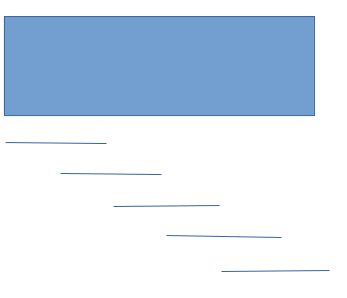
\includegraphics[scale=0.5]{image_mfcc.png}
\end{frame}

\begin{frame}{Feature generation}
GMM supervector $M$~\cite{Reynolds}. 
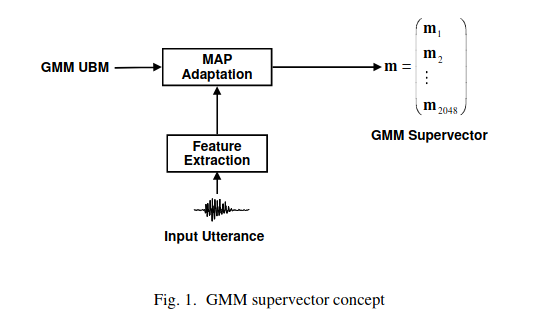
\includegraphics[scale=0.5]{image_supervector.png}
\end{frame}

\begin{frame}{Joint factor analysis}
\begin{itemize}
 \item Classical approach.  Speaker utterance is represented by a supervector
 $$M=m + Ux + Vy.$$
 $V$ defines speaker subspace, $U$ defines session subspace. 
 \item Drawback: channel factors contain information about the speaker.
 \item Total variability space:
 $$M = m + Tw.$$
\end{itemize}
\end{frame}

\begin{frame}{Session variability compensation}
\begin{itemize}
 \item NAP --- Nuissance Attribute Projection.
 \item WCCN --- Within Class Covariance Normalization. 
 \item LDA --- Linear Discriminant Analysis: find features that discriminate speakers best. 
 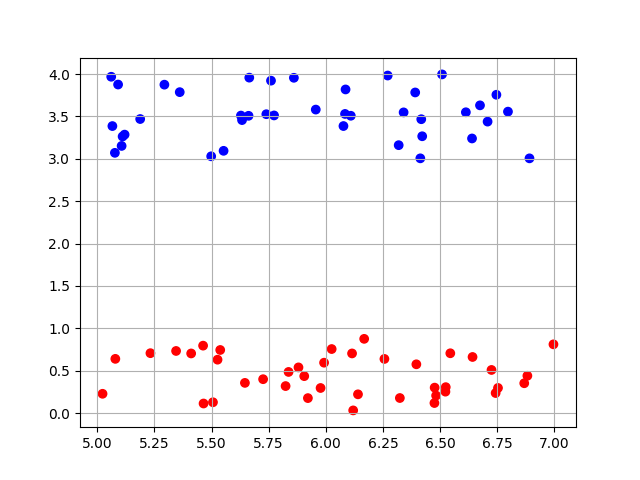
\includegraphics[scale=0.5]{image_scatter.png}
\end{itemize} 
\end{frame}

\begin{frame}{Codecs}
\begin{itemize}
 \item Codecs by sampling frequency:
 NB --- narrow bandwidth (sampling frequency 8kHz), WB --- broad bandwidth (sampling frequency 16 kHz).
 \item Codecs by bit rate: low or high bit rate. 
 \item Codecs with higher bit rate affect speaker recognition less.
 \item NB codecs --- worse recognition effectiveness. 
 \item Some frequency bands more discriminative than others~\cite{Fernandez2014a}.
\end{itemize}
\end{frame}


\begin{frame}{Experiments}
\begin{itemize}
 \item Data transmitted through a digital telephone network.
 \item First experiment: MOS quality measurement for different codecs. t
 \item Second experiment: influence of speech codec on speaker identification.
 4 speakers, 7 codecs. High bit-rate codecs provide better speech quality and preserve better speaker 
 discriminative capacity. 
 \item Third experiment: NIST dataset, use of S-LDA variability compensation. Codecs G.722, GSM 6.20.
 S-LDA method improves speaker recognition. 
\end{itemize}

\end{frame}


\appendix
\section<presentation>*{\appendixname}
\subsection<presentation>*{Literature}

\begin{frame}[allowframebreaks]
  \frametitle<presentation>{Literature}
    
  \begin{thebibliography}{10}
 
  \beamertemplatearticlebibitems

  \bibitem{CodecArt}
    José R. Calvo de Lara, Flavio J. Reyes Diaz, Gabriel Hernández Sierra, Orlando Jimenez Alcazar.
    \newblock A method to compensate the influence of speech codec in speaker recognition.
    \newblock {\em International Journal of Speech Technology}, 2018.
  
    \bibitem{DehakArt}
    Najim Dehak et.al.
    \newblock Front-End Factor Analysis for Speaker Verification.
    \newblock {\em IEEE Transactions on Audio Speech and Language Processing}, 2011.
    
    \bibitem{Fernandez2014a}
    Fernández L., Wagner M., Möller S. 
    \newblock{Advantages of wideband over narrowband channels for speaker verification employing
    MFCCs and LFCCs}. 
    \newblock {\em ISCA Interspeech Conference Proceedings}, 2014.
    
    \bibitem{Reynolds}
    W. M. Campbell, D. E. Sturim, D. A. Reynolds
    \newblock{Support Vector Machines using GMM Supervectors for Speaker Verification}
    \newblock {\em IEEE Signal Processing Letters}, 2006. 
  \end{thebibliography}
  
\end{frame}

\end{document}


